\documentclass[twoside, letterpaper, american]{article}

\usepackage[margin=1in]{geometry}
\usepackage{graphicx}
\usepackage{babel,blindtext}
\usepackage{cleveref}


\begin{document}
\title{42 Winks}
\author{GitHub: JeremySilverTongue}
\date{\today}

\maketitle


\section*{Description}

Sleep tracking has been a common use for smartphones for a long time. However, accelerometer based tracking is unweildly, and requires looking at your phone right before going to sleep. Also there is little evidence that the graphs of sleep cycles that accelerometer trackers generate has anything to do with reality. There's a reason proper sleep studies require the full cyborg treatment.

However, in the spirit that it's hard to improve something you're not measuring, I really still want a way to track my own sleep habits, just by reporting to an app when I go to sleep and wake up. 42Winks (based on the idom ``To catch 40 winks'', plus a couple extra (also, you know, Douglas Adams)) is my idea to fill that need. It is a simple app that allows you to easily log your sleep, see your progress, and collect awesome achievements as you sleep better and better.

\section*{Intended User}

The target user of this product is anyone who wants to simply record how much sleep they're getting. They might be an athlete, a desk warrior, or perhaps someone who believes in the quantified self.

\section*{Features}

The core workflow of this app will allow the user to specify when they intend to go to sleep (e.g. I will go to sleep in 30 minutes, see \cref{fig:sleep}). Then, when rising in the morning, the user will be prompted to say either ``I woke up just now'' or ``I woke up at XX:XX time''. The user can then view a log of previous nights of sleep they have recorded (see \cref{fig:log}. They can view a graph of how long they have slept on previous nights (\cref{fig:graph}. Finally, they can view a trophy case of achievements (for stuff like: first night logged, first night of 8 hours or more, first week hitting 8 hours every night, etc. See \cref{fig:trophy}).

\begin{figure}[!htb]
\minipage{0.49\textwidth}
  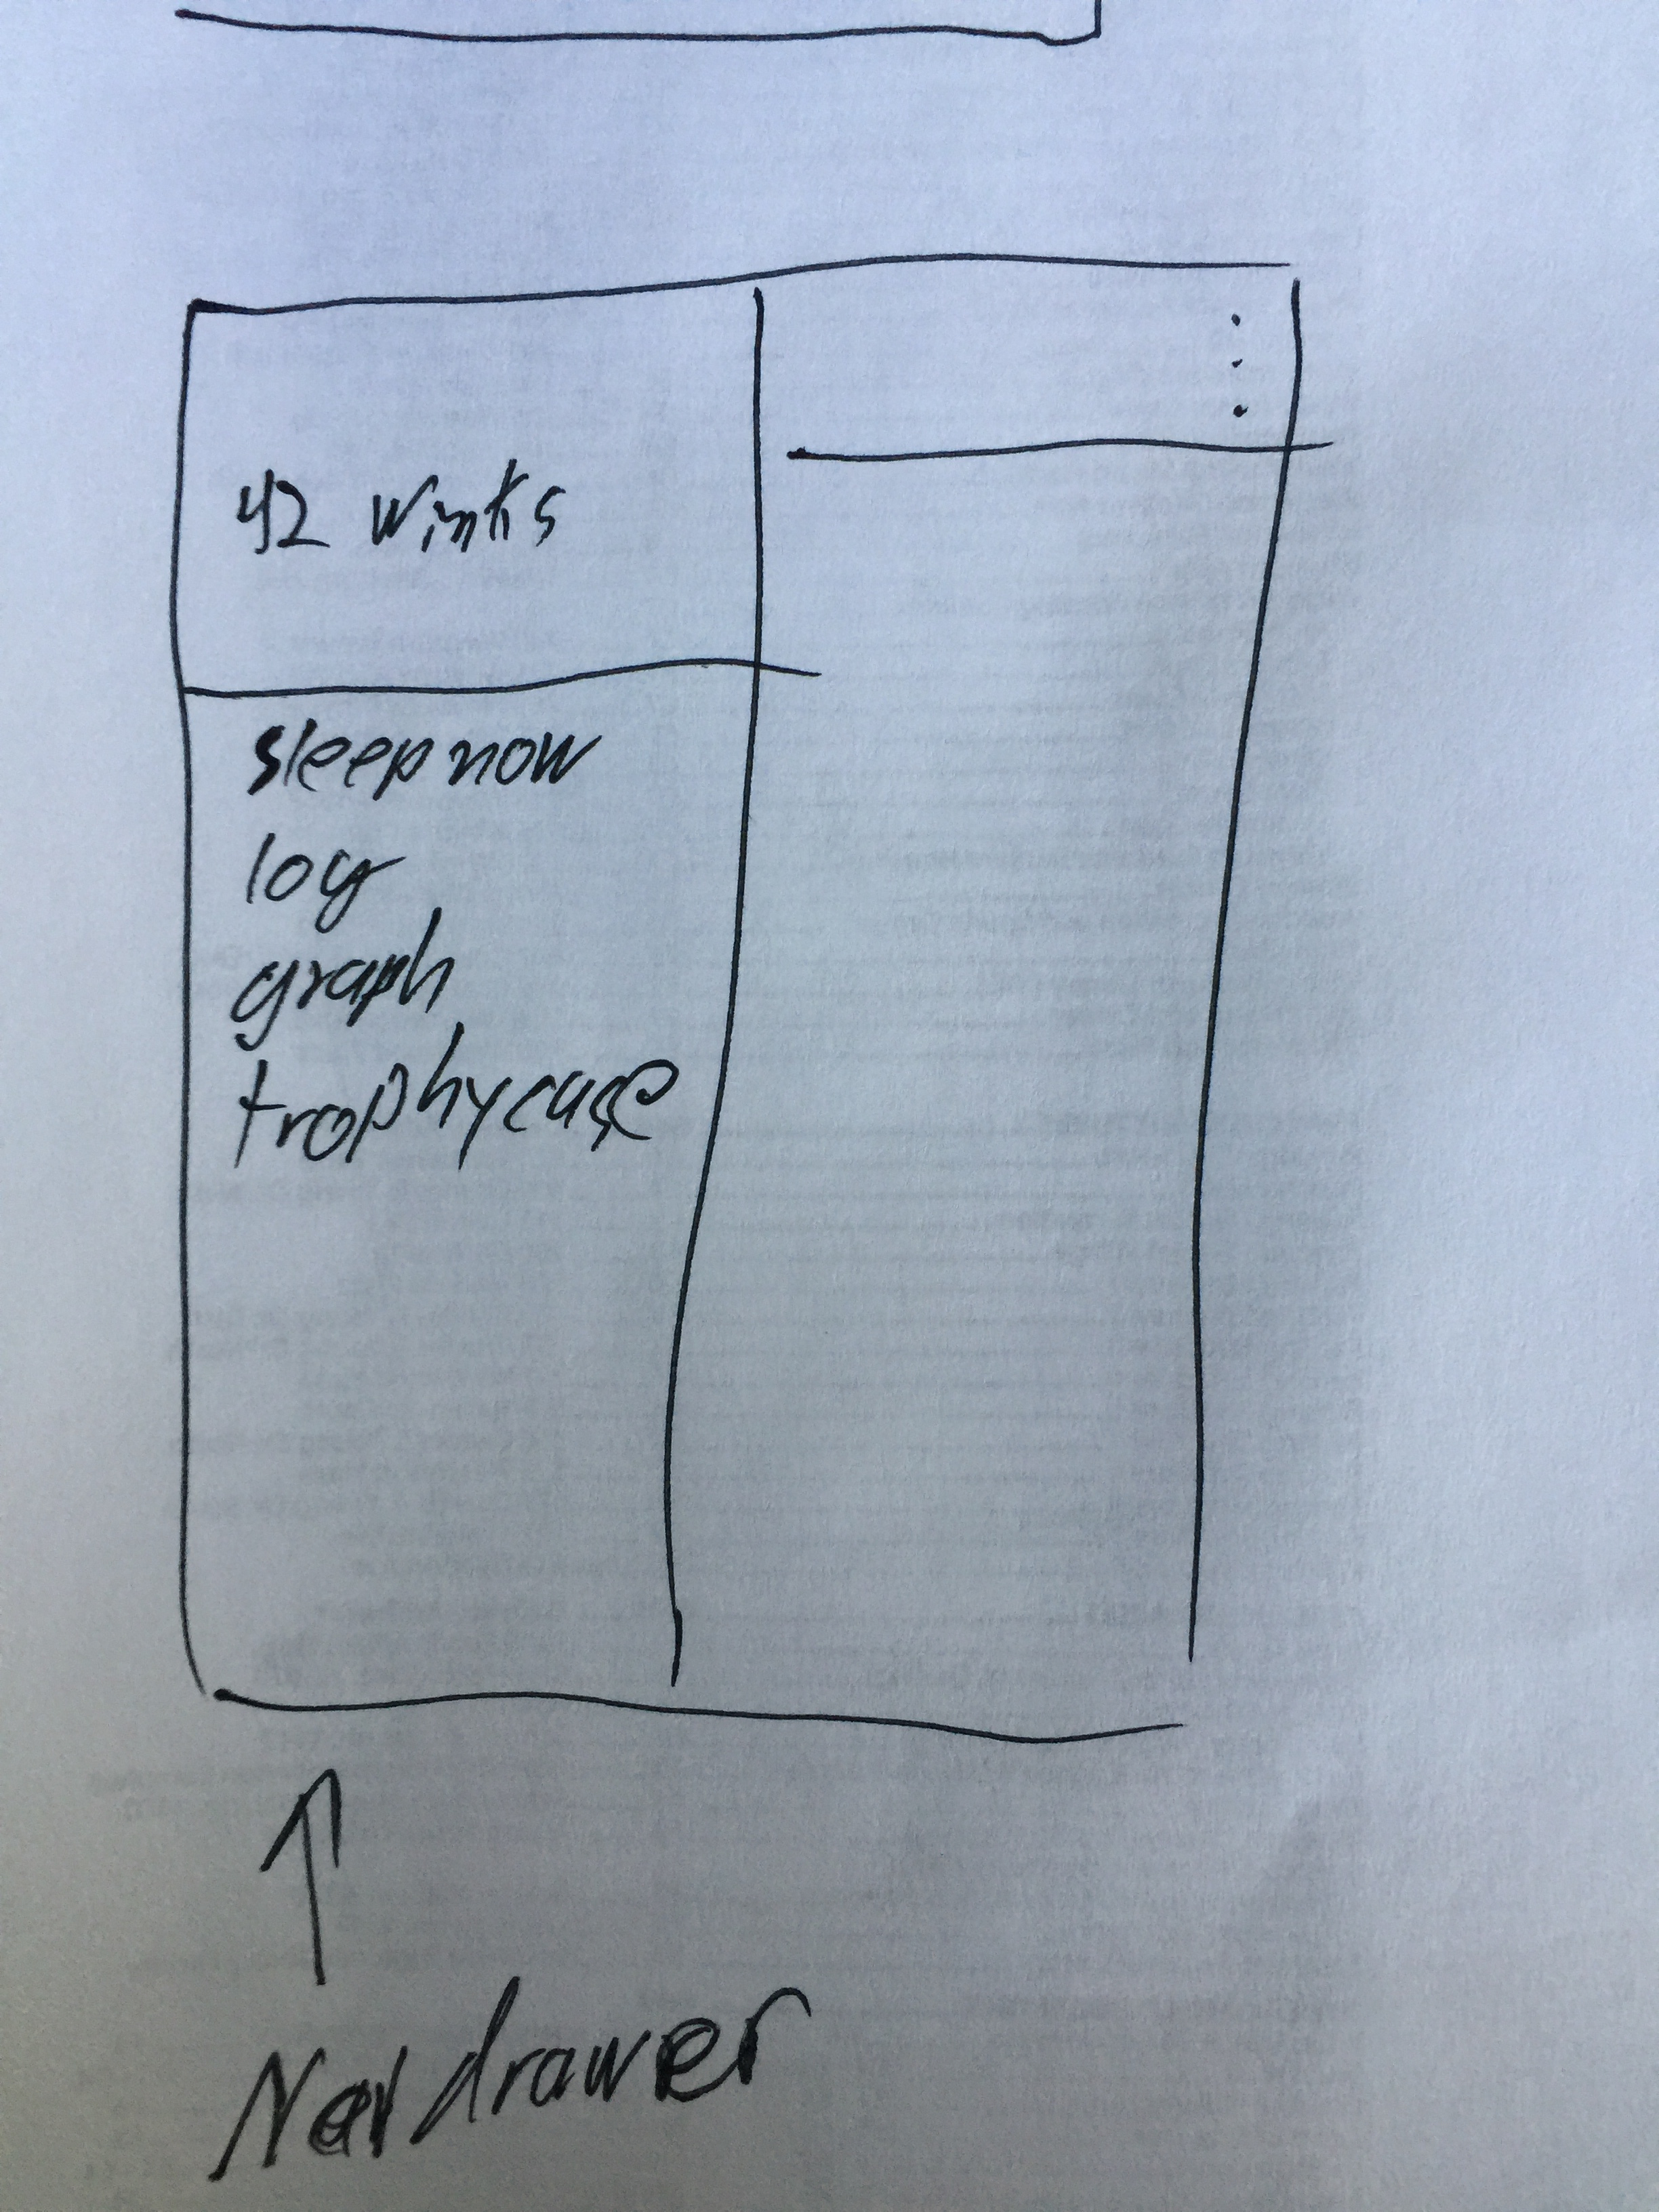
\includegraphics[width=\linewidth]{images/drawer.JPG}
  \caption{A really Awesome Image}\label{fig:drawer}
\endminipage\hfill
\minipage{0.49\textwidth}
  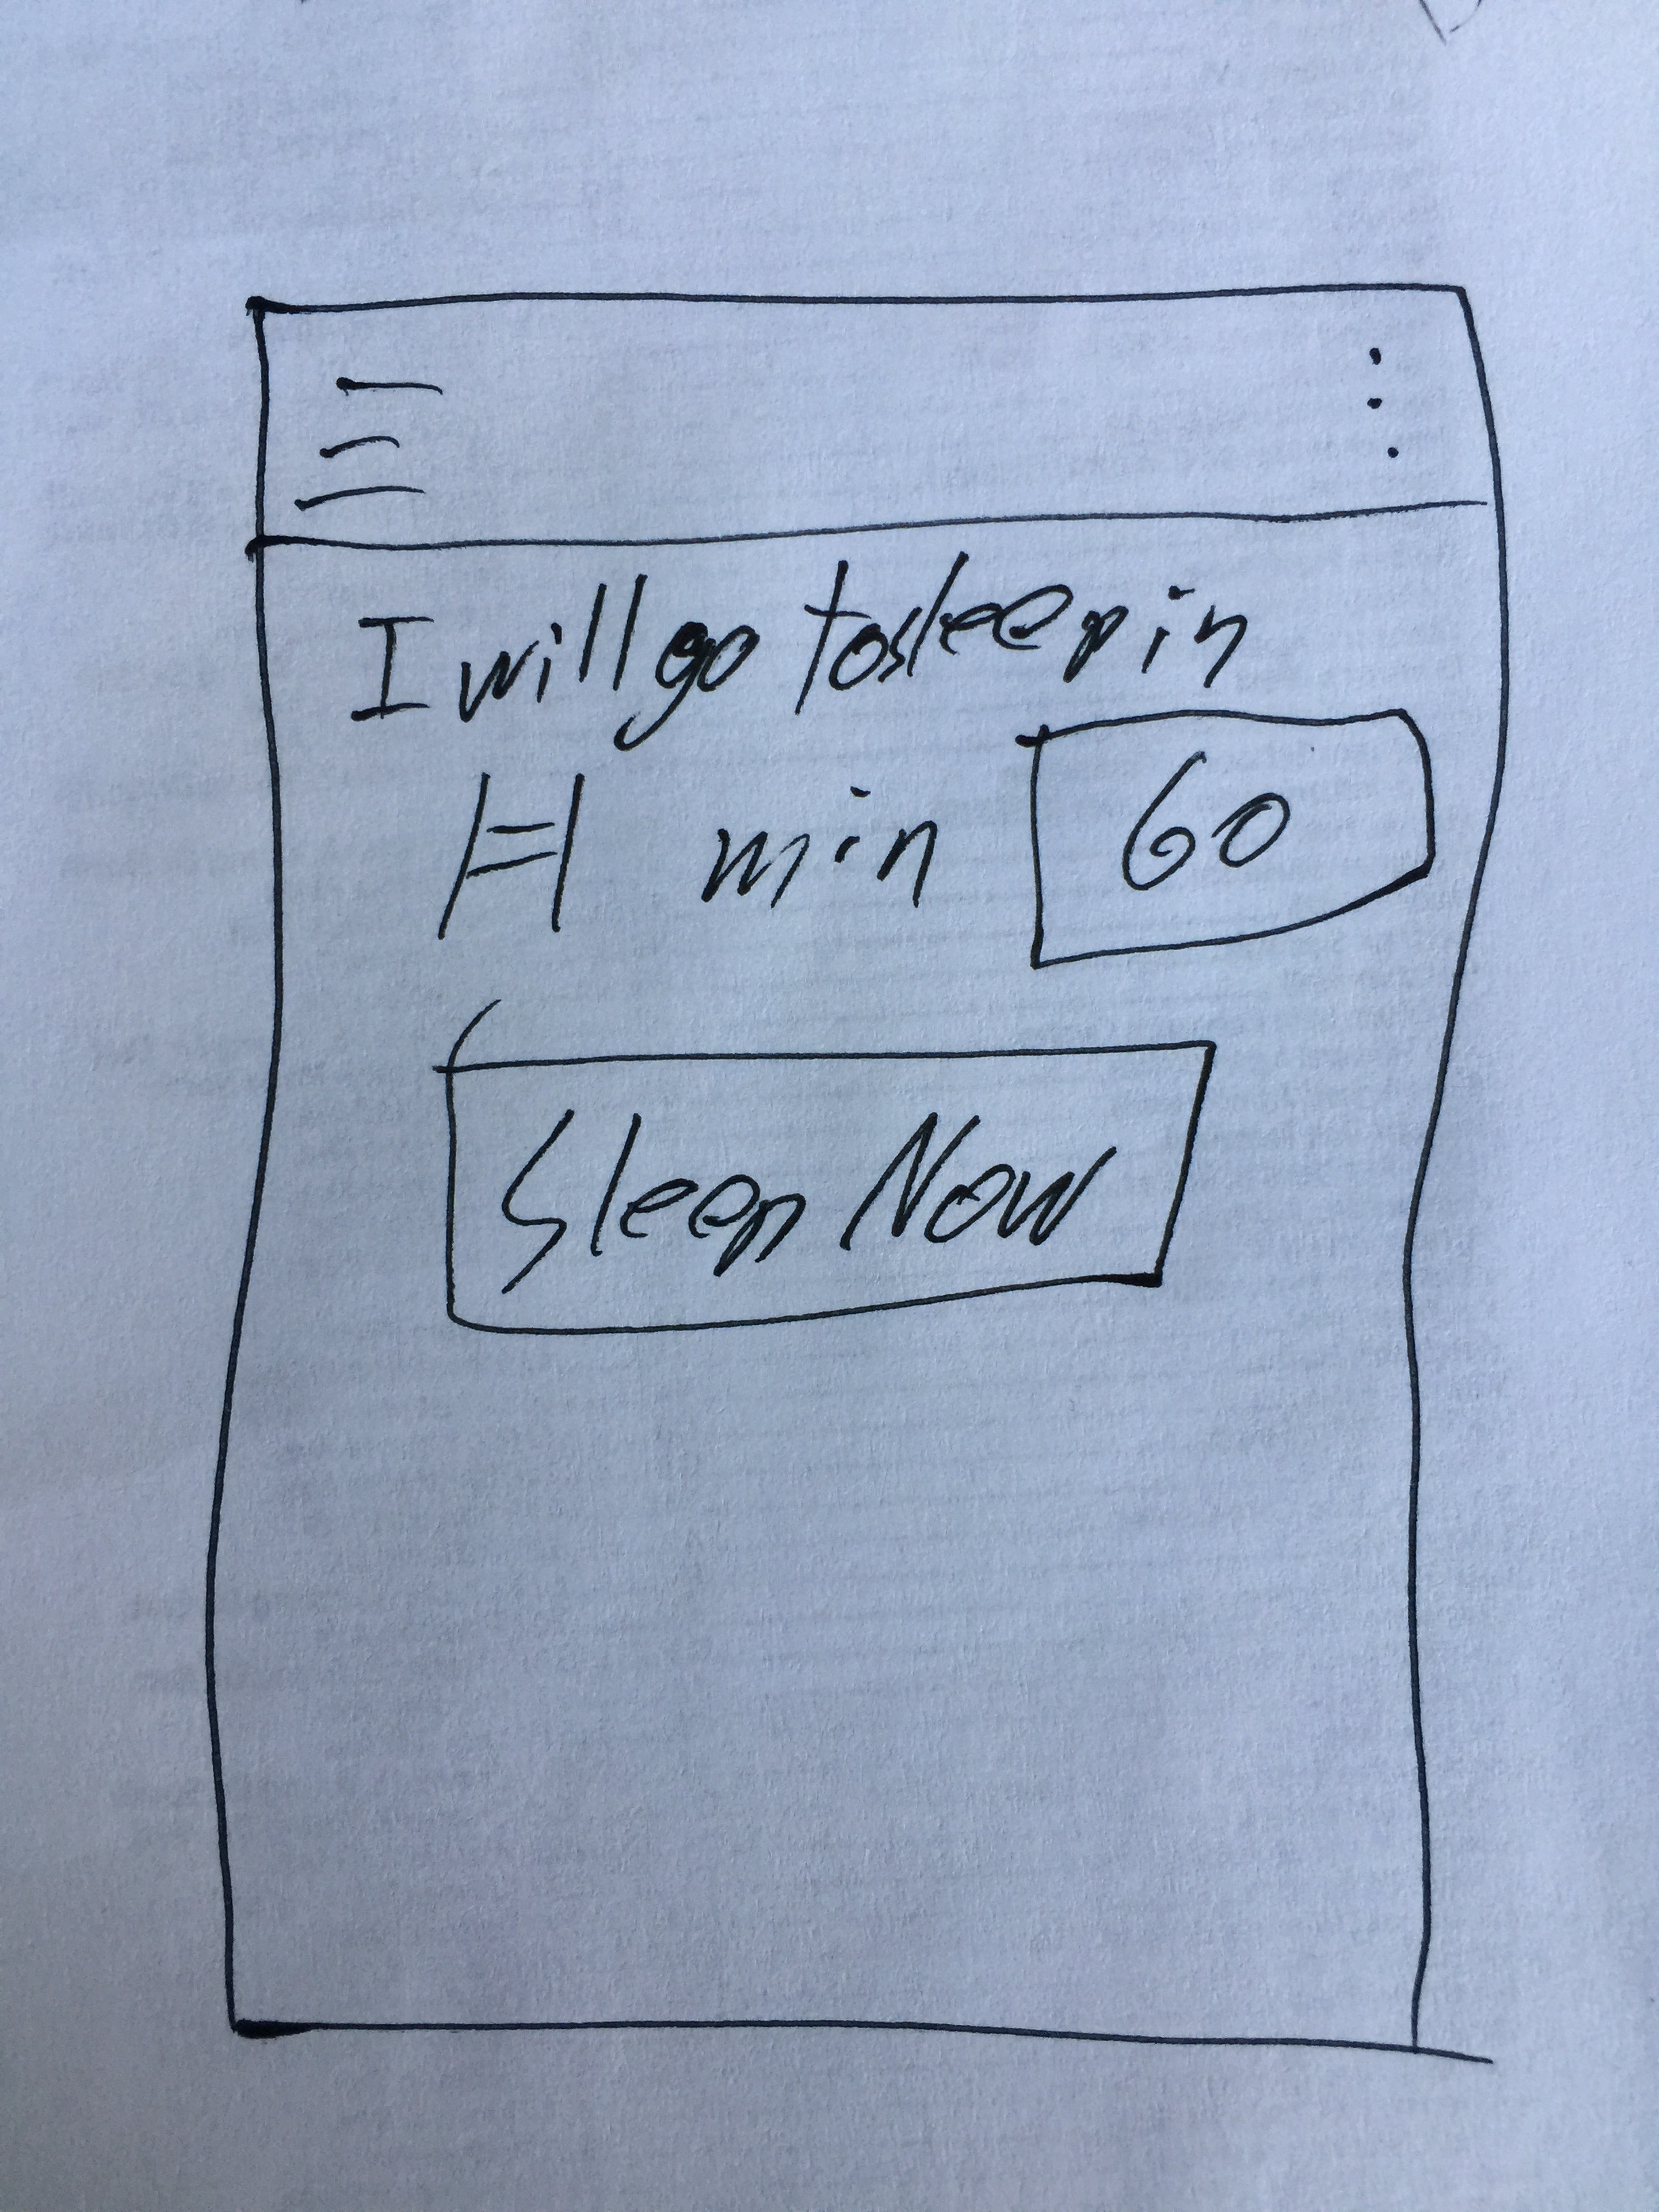
\includegraphics[width=\linewidth]{images/sleep.JPG}
  \caption{A really Awesome Image}\label{fig:sleep}
\endminipage\\\bigskip
\minipage{0.32\textwidth}%
  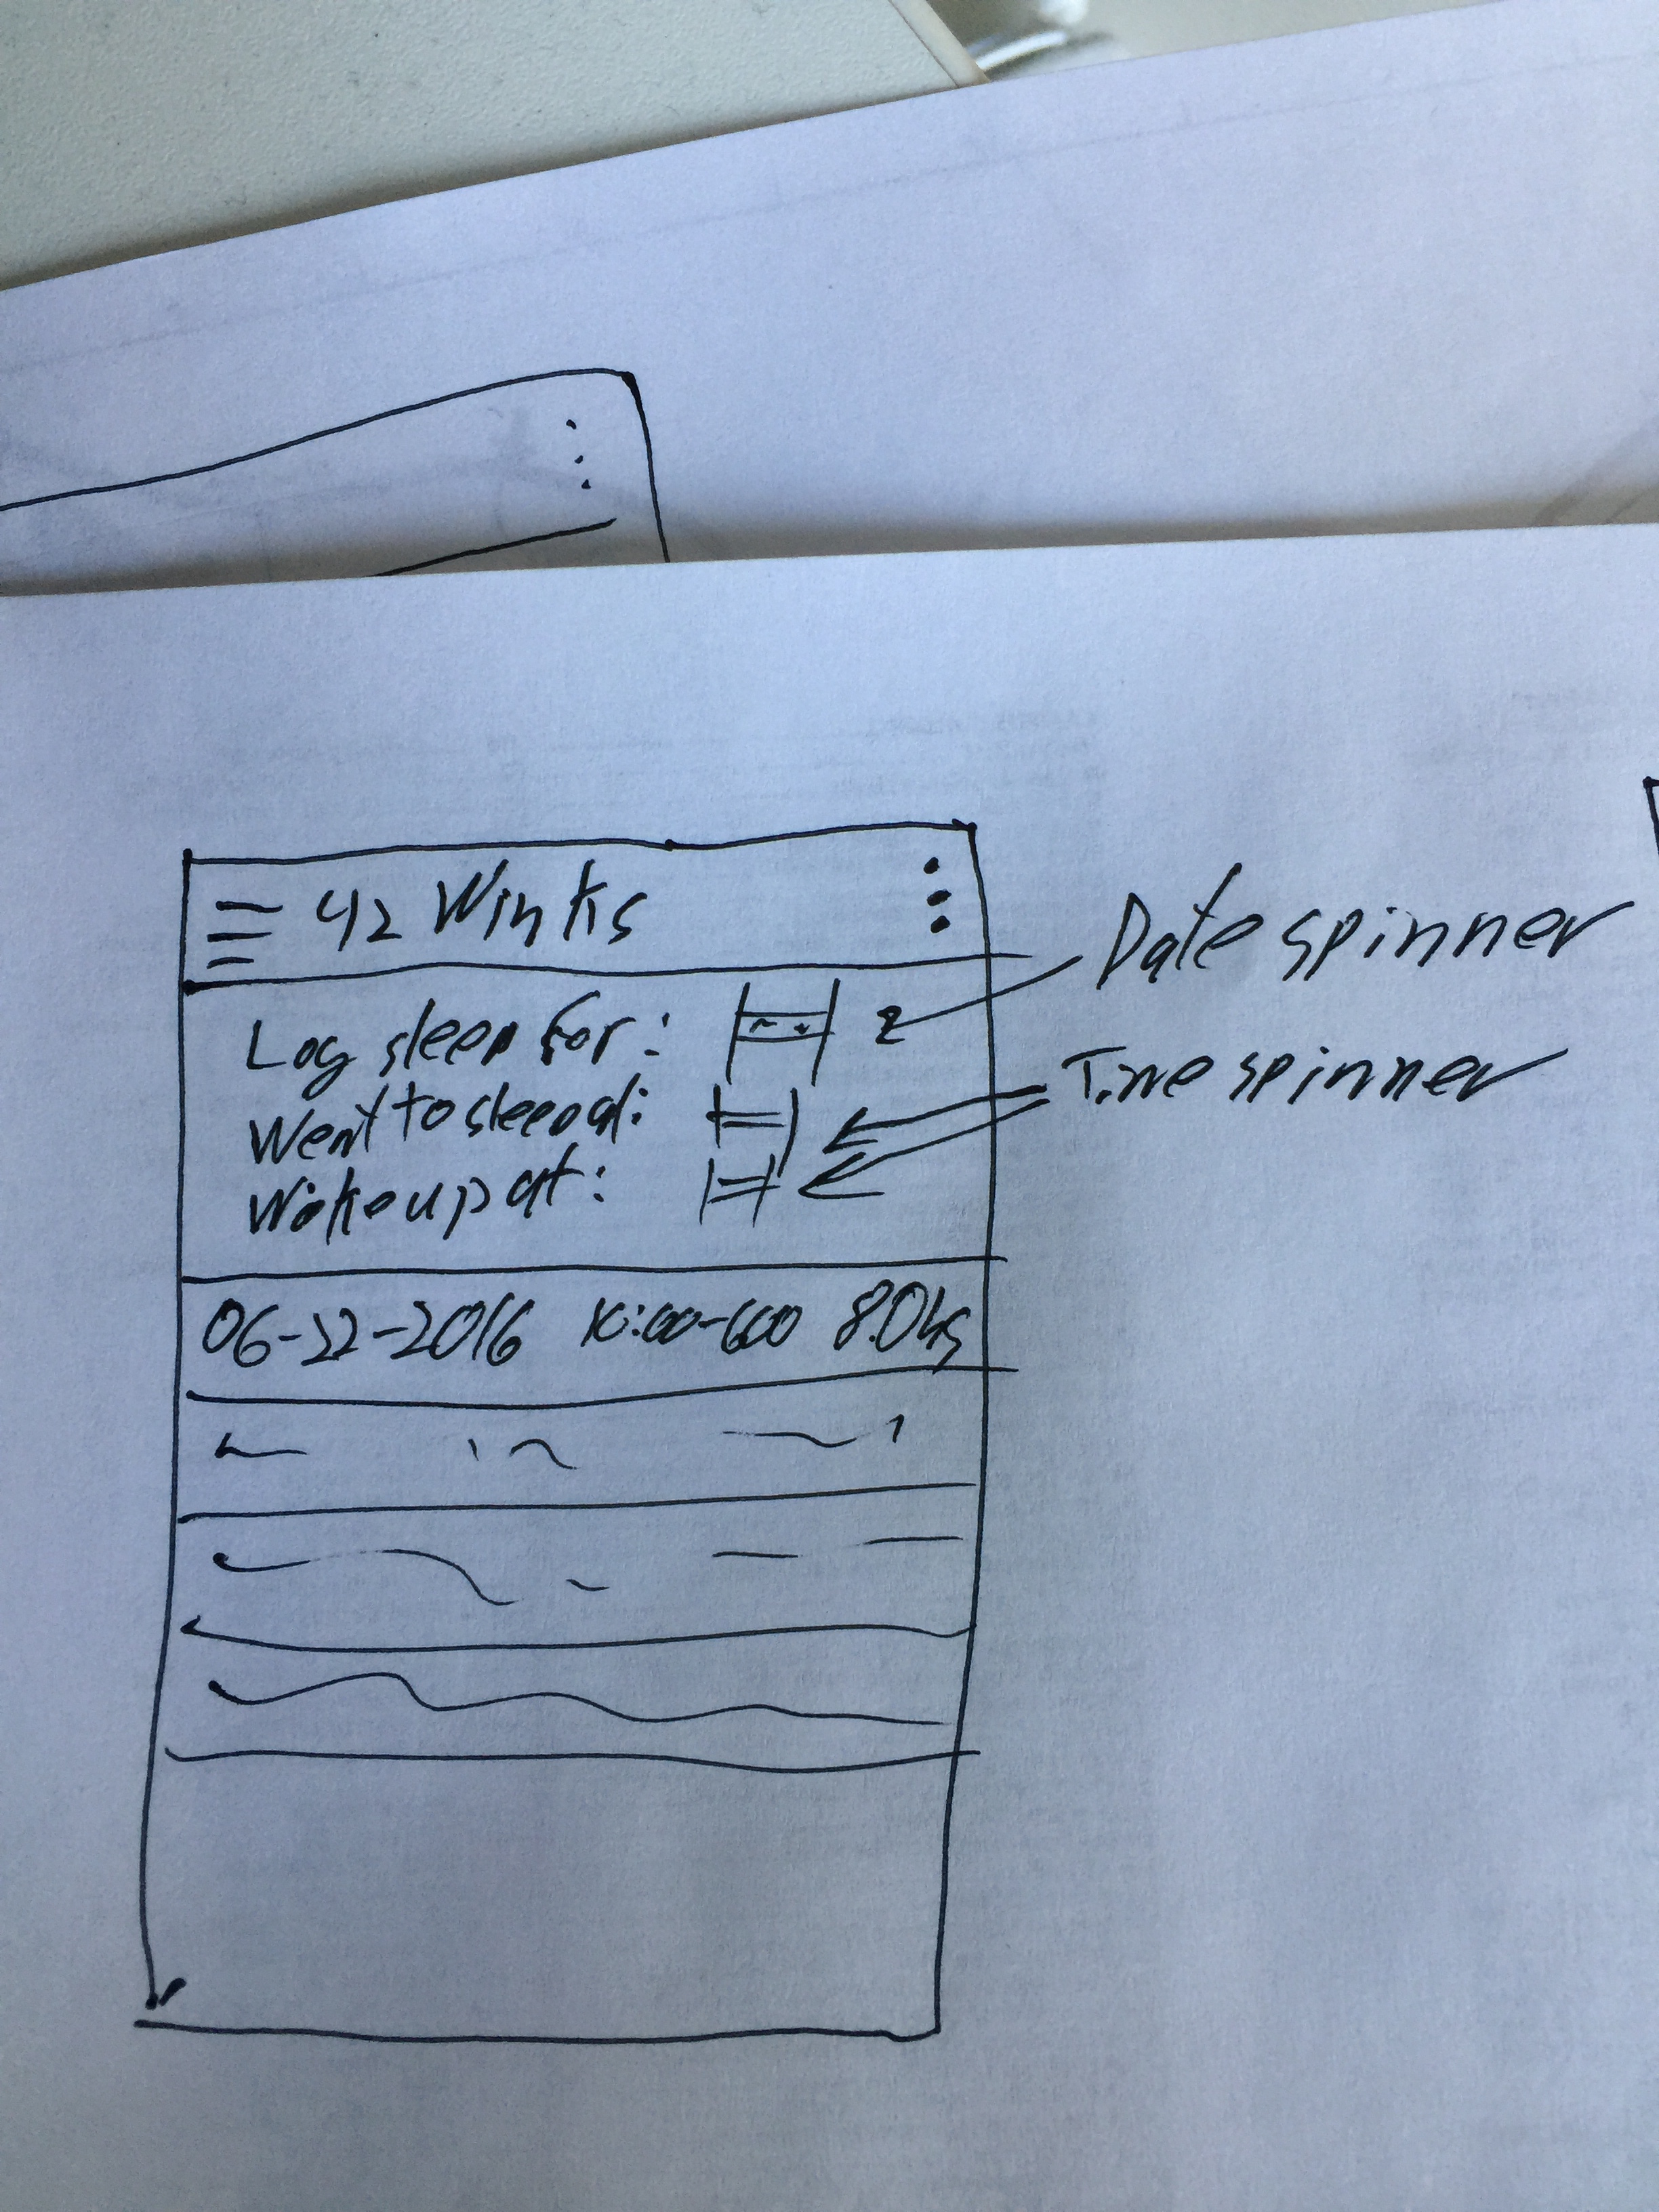
\includegraphics[width=\linewidth]{images/log.JPG}
  \caption{A really Awesome Image}\label{fig:log}
\endminipage\hfill
  \minipage{0.32\textwidth}
  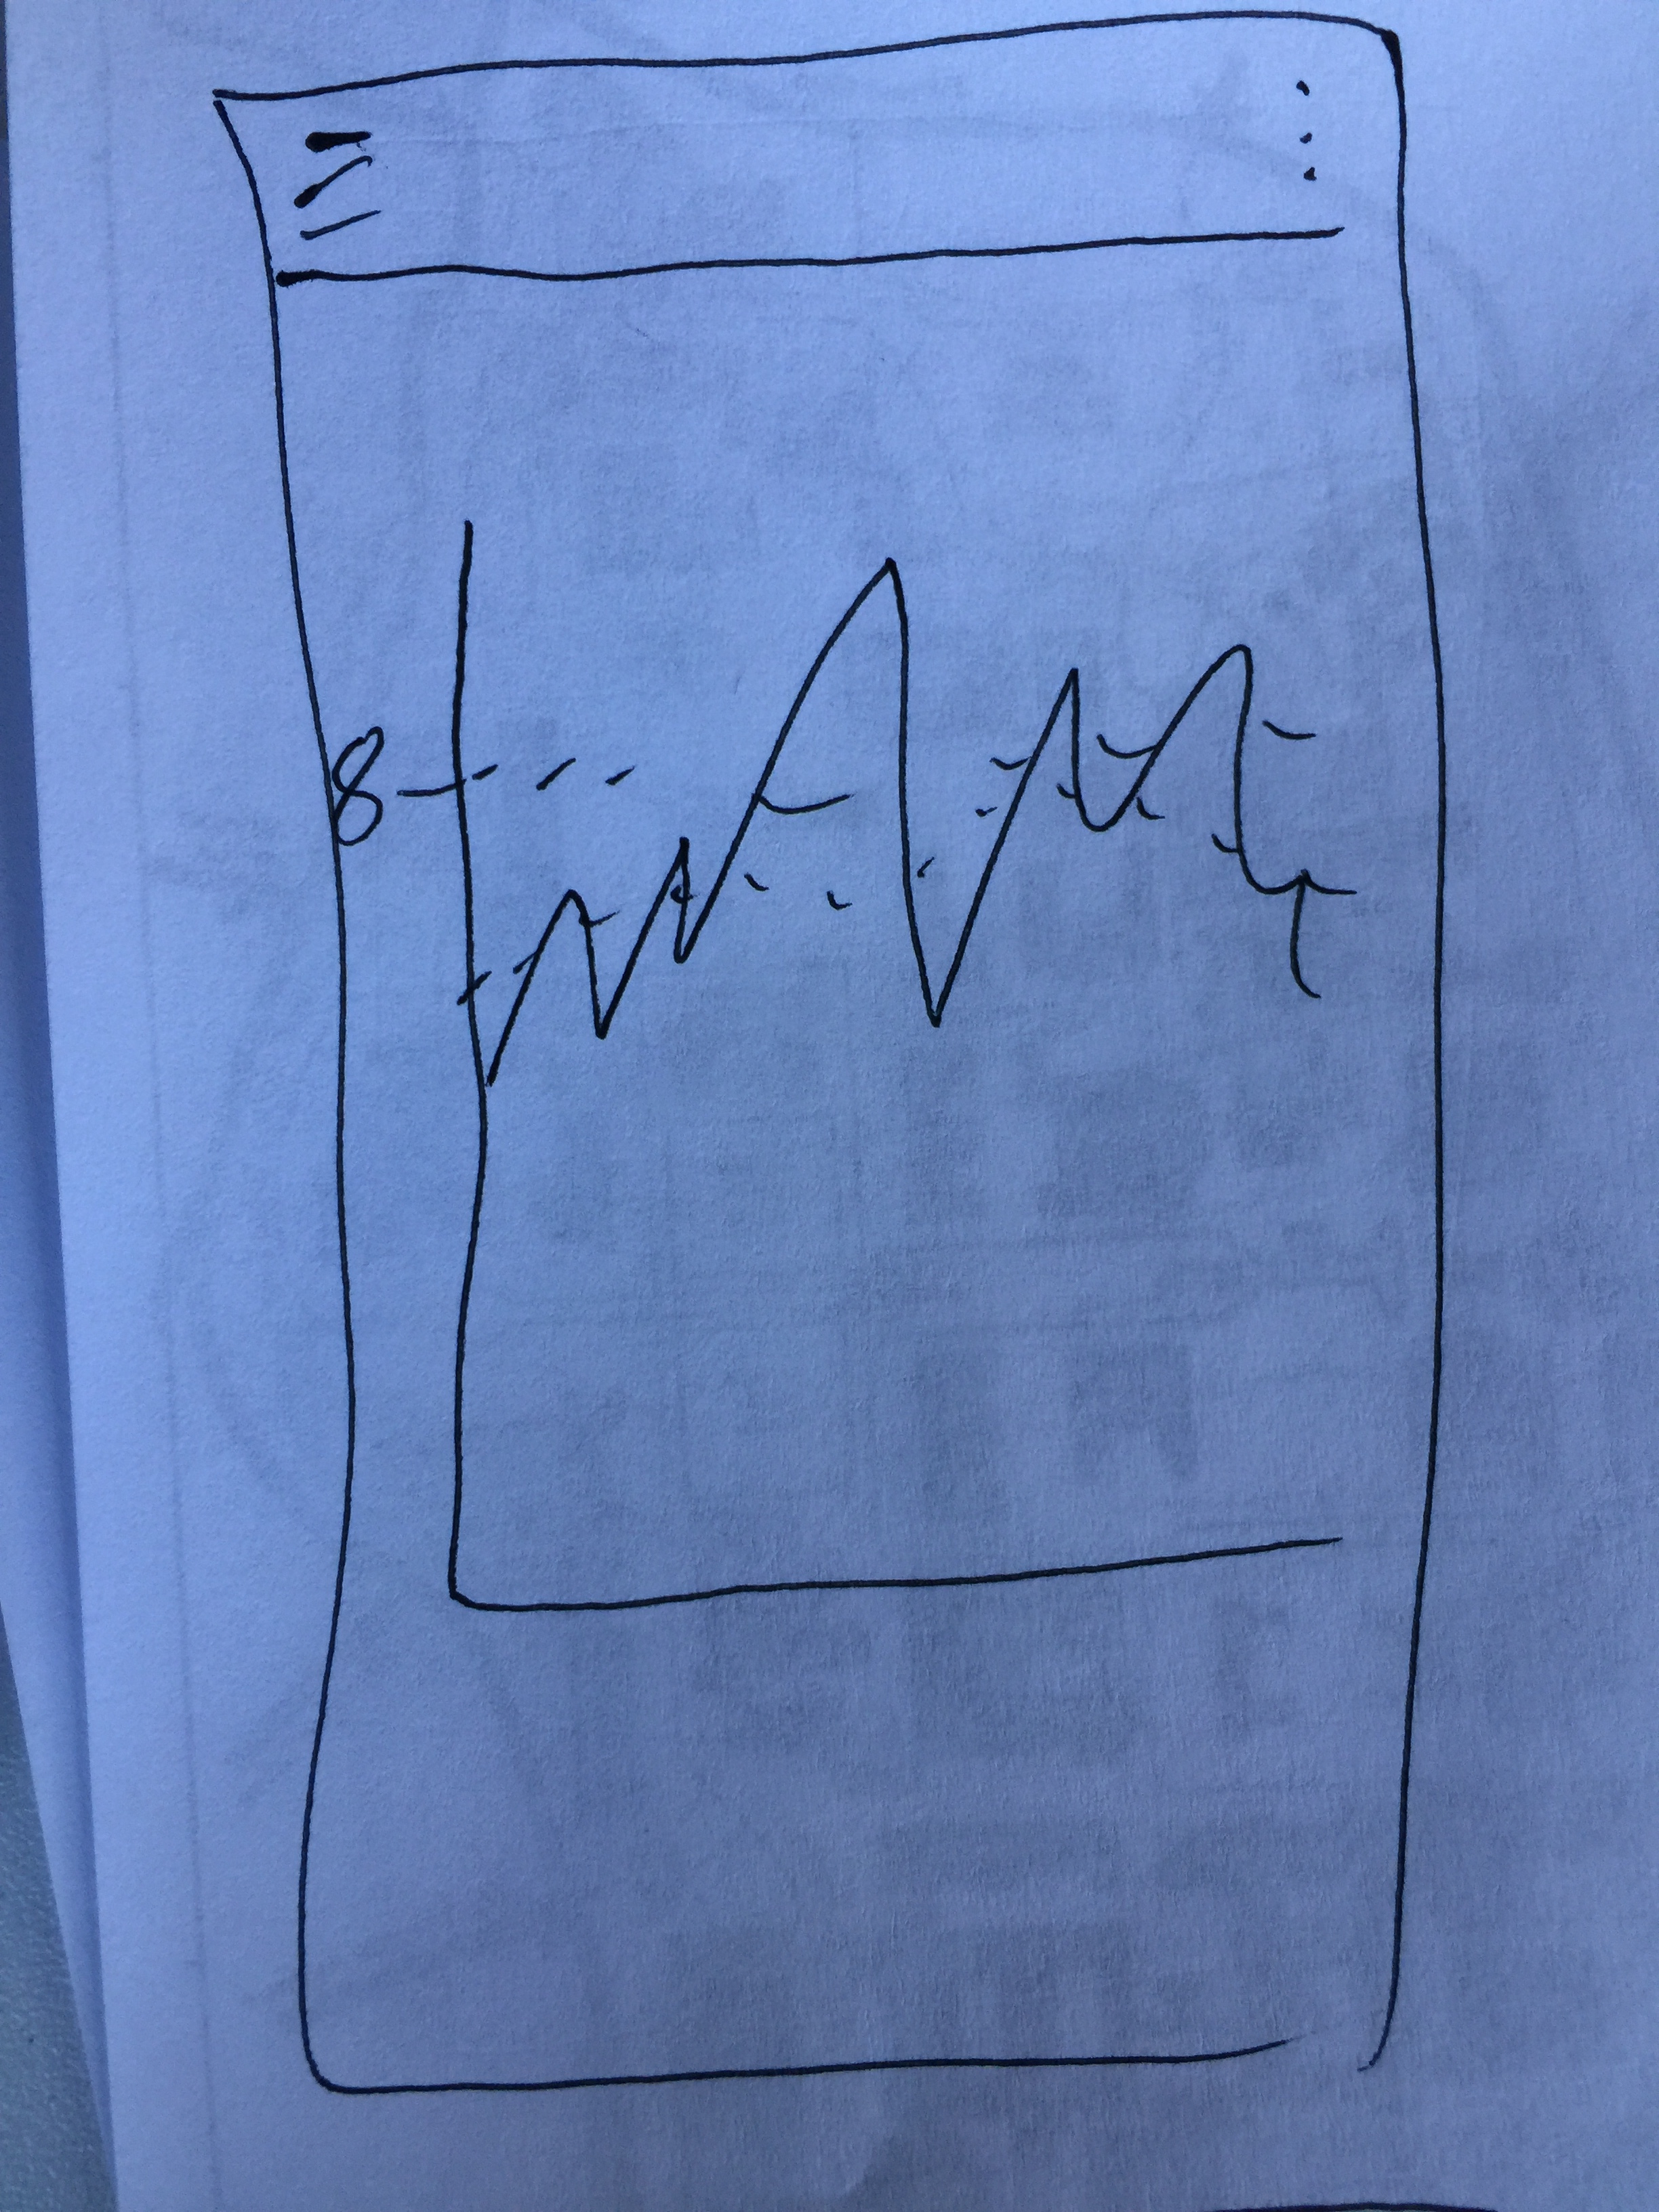
\includegraphics[width=\linewidth]{images/graph.JPG}
  \caption{A really Awesome Image}\label{fig:graph}
\endminipage\hfill
\minipage{0.32\textwidth}
  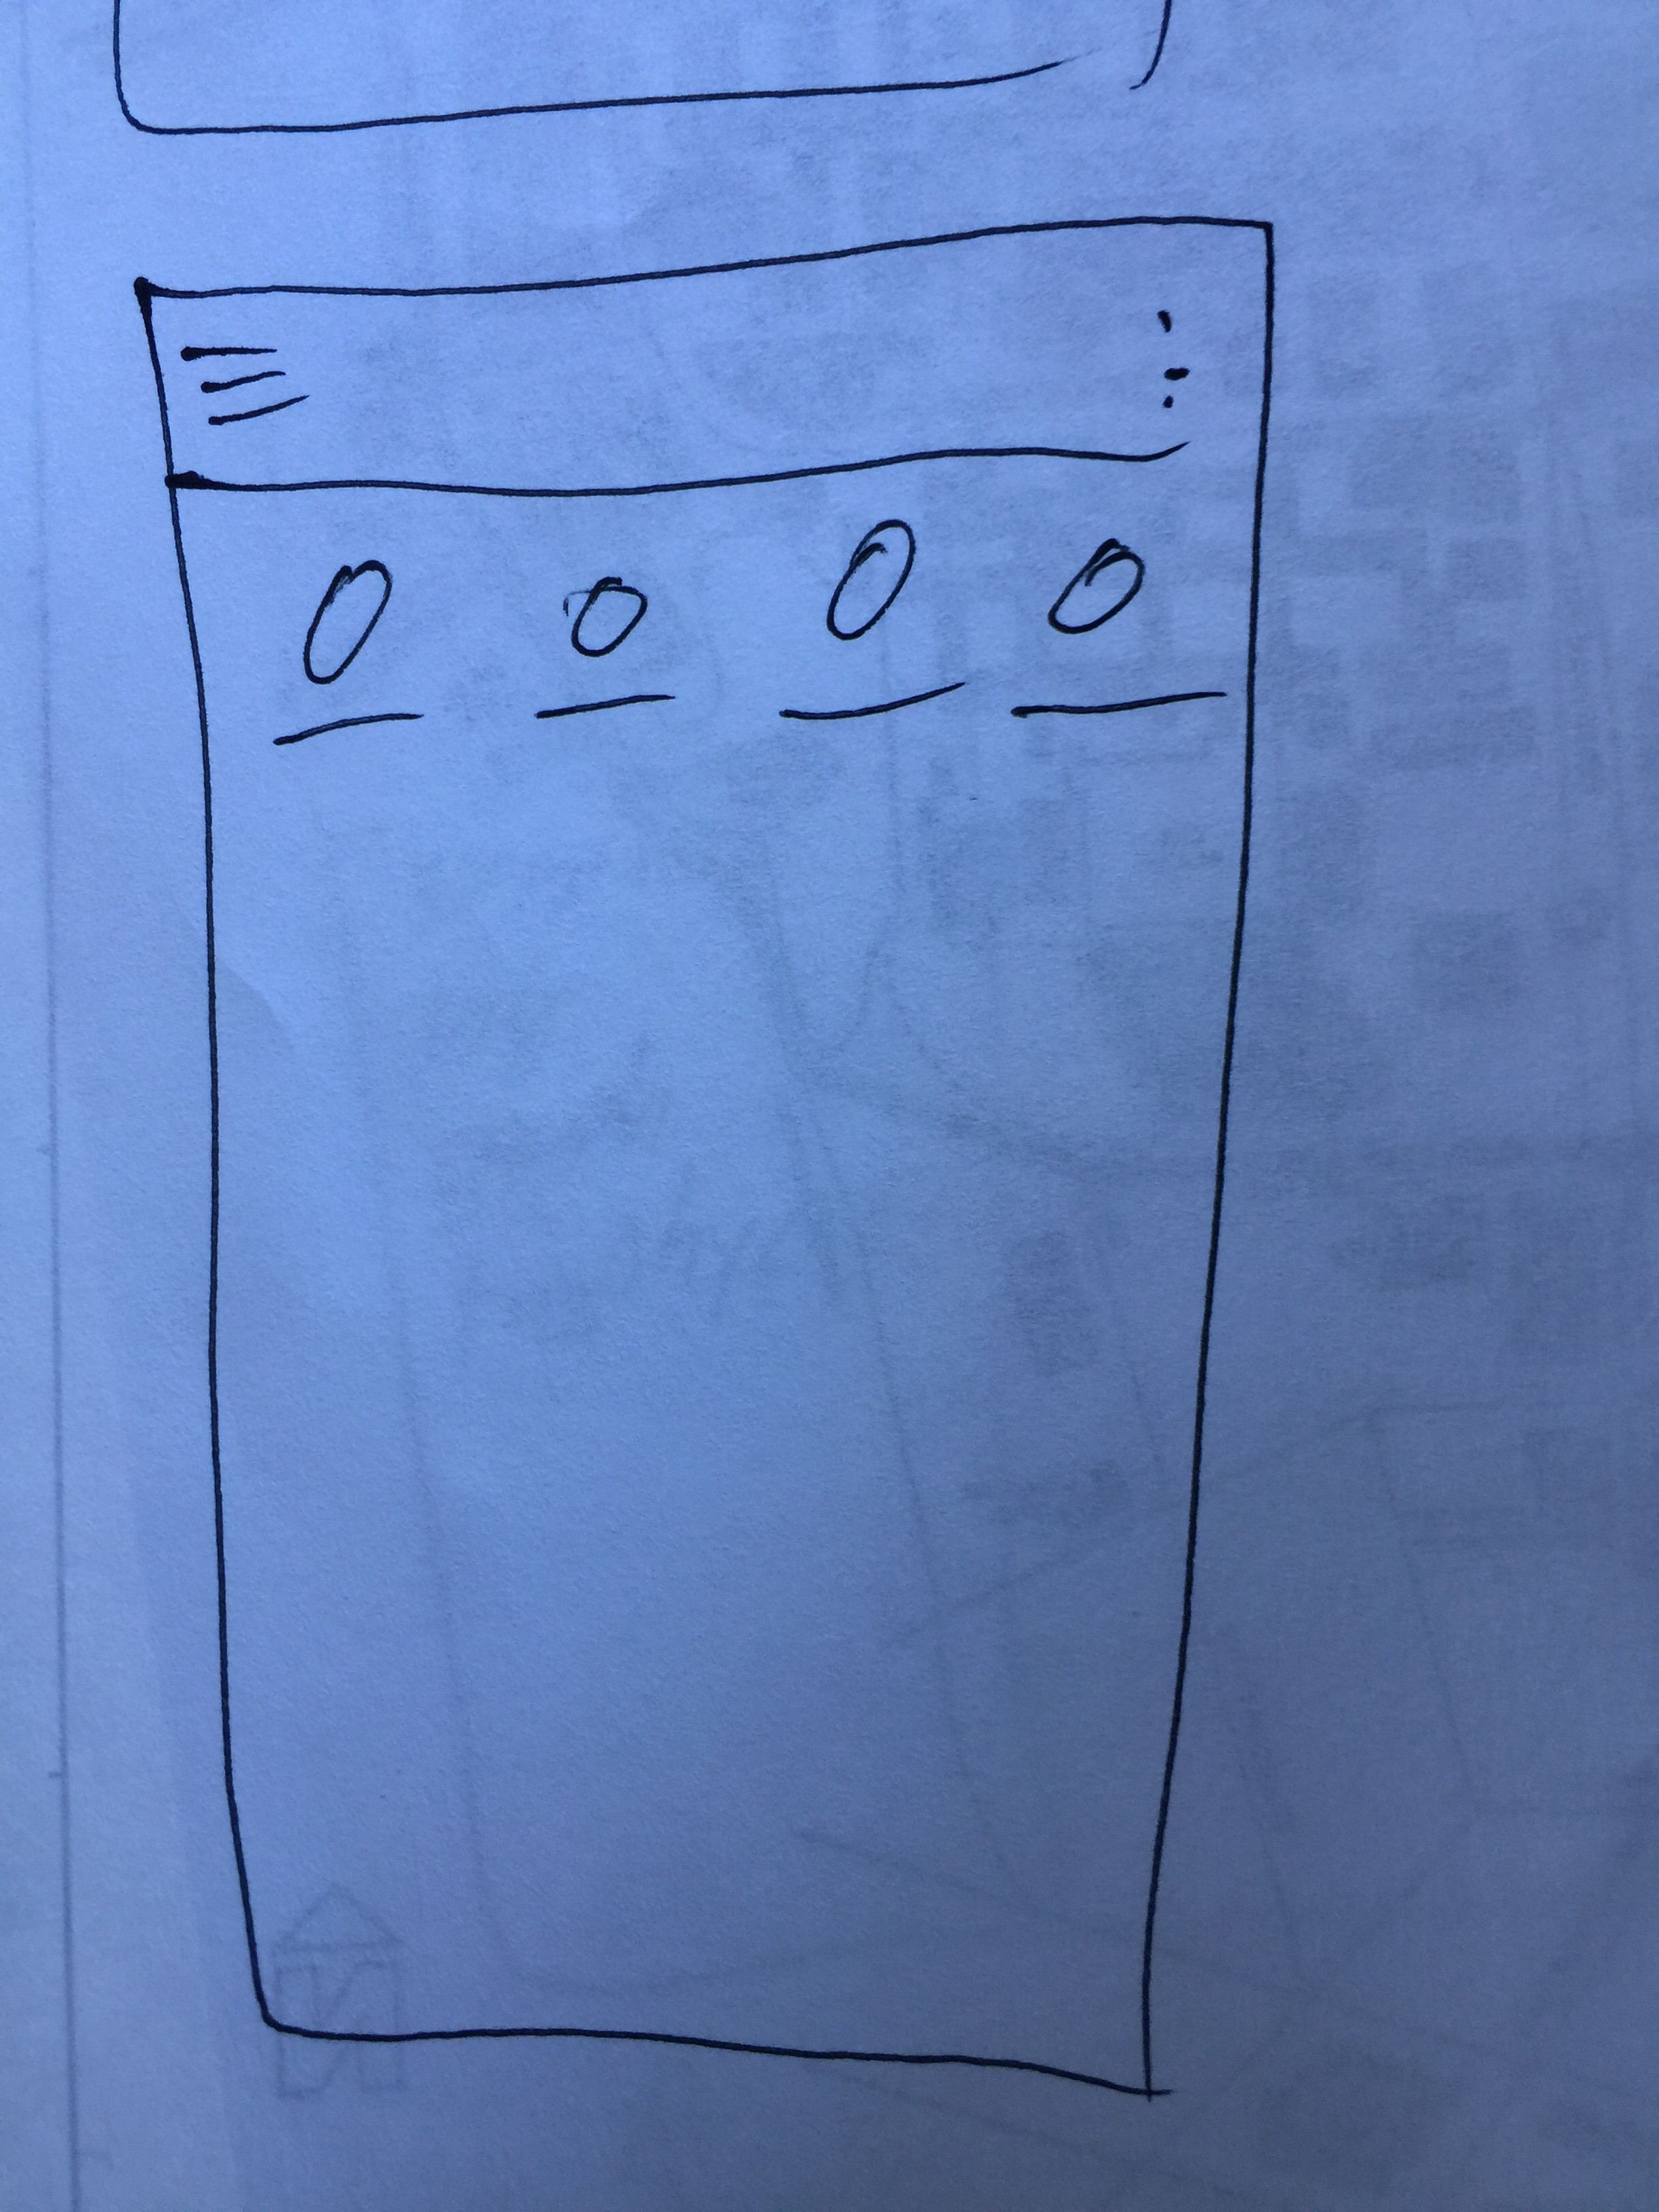
\includegraphics[width=\linewidth]{images/trophy.JPG}
  \caption{A really Awesome Image}\label{fig:trophy}
\endminipage
\end{figure}


\section*{Key Considerations}
\subsection*{How will your app handle data persistence?}

Each night of sleep will be stored as a row in a content provider backed by a SQLite database. Shorter lived information (such as if the user is currently sleeping) will be stored in shared preferences.

\subsection*{Describe any corner cases in the UX}

One thing to deal with is what happens if the user forgets to wake up. I'll notify the user if they've slept for more than 12 hours, and just kill the sleep sesh if it's more thank 24 hours.


\subsection*{Describe any libraries you’ll be using and share your reasoning for including them}

I'll use Timber for logging and and Butterknife for easy view binding. I'll probably be using MPAndroidChart for the graph activity.

\subsection*{Describe how you will implement Google Play Services}

The app will display ads on the Sleep Now screen, and will integrate Google Analytics for auto activity tracking, as well as goal tracking for each of the achievements.


\section*{Next Steps: Required Tasks}

Here's my plan of attack:

\begin{description}

\item[Project Setup] Already done for the most part. Just firing up a new project with a Nav Drawer activity and adding in the various libraries I'm using.

\item[Persistance Setup] The next step will be setting up the database and content providers.

\item[Log Screen] The log screen provides all the core funtionality, allowing the user to add and delete records. Thus I'll tackle it first.

\item[Graph Screen] The graph screen should be pretty easy, given the similarity to the assigned task bask in Stock Hawk.

\item[Sleep Now Screen] The sleep now screen should be pretty straight forward.

\item[Persistant Notification] I'll create a persistant notificaiton to be displayed when the user is sleeping, reminding them to record when they stop sleeping.

\item[Trophy Case] Next I'll create the trophy case, the logic for determining what achievements the user has earned, and the Google Analytics integration to track what users are getting which achievements.

\item[Widget] Finally, I'll add a widget that allows the user to start and stop sleeping.

\end{description}


\end{document}